\subsubsection{UC21 - Visualizzazione lista delle funzioni di proprietà dell’utente}
\begin{figure}[h]
	\centering
	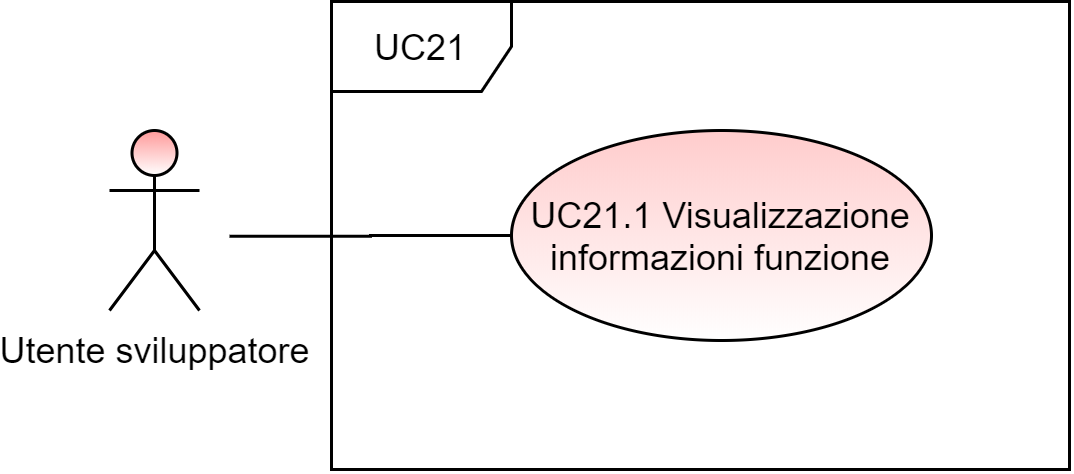
\includegraphics[scale=\ucs]{./res/img/UC21.png}
	\caption {UC21 - Visualizzazione lista funzioni di proprietà dell’utente}
\end{figure}
\begin{itemize}
	\item \textbf{Attori primari:} \us{};
	\item \textbf{Attori secondari:} \re{};
	\item \textbf{Descrizione:} l’utente richiede la visualizzazione della lista di tutte le funzioni di sua proprietà eseguendo il comando \plista{}. Il sistema stampa a video tale lista;
	\item \textbf{Scenario principale:} 
	\begin{itemize}
		\item l’utente inserisce correttamente ed esegue il comando \plista{};
		\item viene visualizzata la lista di tutte le funzioni di proprietà dell’utente. 
	\end{itemize}
	\item \textbf{Estensioni:} 
	\begin{itemize}
		\item \textbf{UC23:} l’utente non ha ancora pubblicato alcuna funzione, di conseguenza viene visualizzato un messaggio di avviso. 
	\end{itemize}
	\item \textbf{Precondizione:} l'utente inserisce correttamente ed esegue il comando \plista{};
	\item \textbf{Postcondizione:} la CLI\ped{\textit{G}} riporta la lista di tutte le funzioni di proprietà dell’utente. 
\end{itemize}